%% Paper 4 — Meta-learning for cross-basin landslide susceptibility transfer
%% Target journal: Remote Sensing of Environment (Elsevier)
%% Template: elsarticle (same template works for RSE, ISPRS J, RSASE, etc.)

\documentclass[preprint,12pt,3p,authoryear]{elsarticle}

% Standard packages
\usepackage{amssymb}
\usepackage{amsmath}
\usepackage{graphicx}
\usepackage{booktabs}
\usepackage{multirow}
\usepackage{hyperref}
\usepackage{xcolor}
\usepackage{siunitx}       % SI units
\usepackage{adjustbox}     % wide tables
\usepackage{caption}
\usepackage{subcaption}

% Hyperref colors
\hypersetup{
    colorlinks=true,
    linkcolor=blue!50!black,
    citecolor=blue!50!black,
    urlcolor=blue!50!black,
    breaklinks=true,
}

% Figure path
\graphicspath{{../figures_pub/out/}}

% Journal label (changeable depending on submission)
\journal{ISPRS Journal of Photogrammetry and Remote Sensing}

\begin{document}

\begin{frontmatter}

\title{Meta-learning for cross-basin landslide susceptibility transfer across 14 Chilean watersheds: a remote sensing benchmark under spatial cross-validation}

%% Authors
\author[usach]{Francisco Parra\corref{cor1}\fnref{orcid1}}
\ead{francisco.parra.o@usach.cl}
\cortext[cor1]{Corresponding author}
\fntext[orcid1]{ORCID: 0009-0006-0435-1854}

\author[unsl]{Verónica Gil-Costa}
\author[usach]{Carolina Bonacic}
\author[usach]{Mauricio Marín}

\affiliation[usach]{organization={Departamento de Ingeniería Informática, Universidad de Santiago de Chile},
            addressline={Av. Víctor Jara 3659},
            city={Santiago},
            postcode={9170125},
            country={Chile}}

\affiliation[unsl]{organization={Departamento de Informática, Facultad de Ciencias Físico Matemáticas y Naturales, Universidad Nacional de San Luis -- CONICET},
            city={San Luis},
            country={Argentina}}

%% Abstract
\begin{abstract}
Earth-observation data enable landslide susceptibility mapping in mountains, but in \emph{newly-studied} basins the cost of local inventories is prohibitive and models from data-rich basins transfer poorly across geological-climatic gradients. We present the first cross-basin benchmark of first-order meta-learning (Reptile and First-Order MAML, FOMAML) for landslide susceptibility across 14 Chilean watersheds spanning an extreme hyper-arid Atacama (Tilviche-Loa, $\sim$1\,mm/yr) to hyper-humid Patagonia (Magallanes, $\sim$2{,}630\,mm/yr) gradient over 27$^\circ$ of latitude, with features from Sentinel-2, MERIT-DEM, GLCM texture, and WorldClim on a 30\,m grid. We meta-train on 10 sources and evaluate $K$-shot transfer ($K \in \{1, 5, 10, 20\}$) on 4 targets via 24{,}000 adaptations under random and spatial cross-validation, with bootstrap 95\% confidence intervals. Under spatial cross-validation, meta-learning (Reptile or FOMAML) outperforms an Independent baseline at $K=1$ in all four targets, with a mean lift of $+5.5$\,percentage points (pp) $F_1$ and overlapping CIs between Reptile and FOMAML. The advantage decays monotonically and vanishes by $K=20$; meta-learned initializations reach $F_1 \approx 0.78$ within $\leq 3$ gradient steps. A Domain-Adversarial Neural Network baseline does not improve over Independent and underperforms by $-6$\,pp in the smallest target (Copiap\'o, $N=19$). Classical machine-learning baselines reach competitive peak $F_1$ at $K \geq 5$: meta-learning's principal benefit is rapid adaptation efficiency, not absolute discrimination. Source--target climate distance does not predict transfer success ($r=0.01$), suggesting the prior captures generic geomorphic rather than climate-specific signals. The framework applies to low-resource Earth-observation transfer in mountain-hazard monitoring across Latin America.
\end{abstract}

%% Highlights (3-5 bullets, max 85 chars each)
\begin{highlights}
\item First cross-basin meta-learning benchmark for landslide susceptibility in 14 basins.
\item Meta-learning beats the Independent baseline at K=1 in 4/4 targets (spatial CV).
\item Mean +5.5 pp F1 lift (up to +7.8 pp); Reptile and FOMAML within overlapping CIs.
\item DANN underperforms by 6 pp F1 in the smallest target (Copiap\'o, N=19).
\item Climate distance does not predict transfer success---meta-learning is robust.
\end{highlights}

%% Keywords
\begin{keyword}
meta-learning \sep landslide susceptibility \sep transfer learning \sep
remote sensing \sep spatial cross-validation \sep few-shot learning \sep Andes
\end{keyword}

\end{frontmatter}

%% ============================================================
\section{Introduction}
\label{sec:intro}

% TODO: Convert from paper_draft.md section 1
% Hook: data-scarcity problem in newly-studied basins
% Two existing strategies: transfer learning, domain adaptation
% Meta-learning paradigm + gap in landslide literature
% 4 contributions

Remote sensing has reshaped landslide susceptibility mapping by delivering globally consistent inputs: Sentinel-1 C-band SAR products for surface-deformation and amplitude features \citep{poggi2026sentinellandslide}, Sentinel-2 multi-spectral composites for surface cover and vegetation indices, MERIT and Copernicus 30~m DEMs for topographic and hydrologic derivatives, and WorldClim 2.1 bioclimatic surfaces for environmental context. These data, harmonized to a common grid, feed the dominant paradigm of fitting a machine-learning classifier to a per-basin inventory of labeled events---a workflow that produces strong results when local training data are abundant \citep{reichenbach2018review, merghadi2020ml, ma2025metalsm}. However, the practitioner facing a \emph{newly-studied} basin confronts a data-scarcity bottleneck: digitizing a usable inventory typically requires expert geomorphological mapping over hundreds of events, an effort that can take months and is rarely funded for individual watersheds. As a result, basins with sparse inventories ($N<50$ mass-movement records) cannot benefit from data-hungry deep learning approaches, while transfer of models trained on data-rich neighboring basins suffers from systematic shifts in geology, climate, and surface cover \citep{zhu2026thawsusceptibility}.

Two strategies have emerged to mitigate this. \textbf{Transfer learning} by fine-tuning a model pre-trained on data-rich basins \citep{ghorbanzadeh2022landslide} reduces label requirements but still needs tens to hundreds of target samples. \textbf{Domain adaptation} approaches such as DANN \citep{ganin2015dann} attempt to learn domain-invariant representations from labeled source data and unlabeled target data, with mixed success in remote sensing \citep{tuia2016domain, huang2026transferability}; recent work on source-free domain adaptation for cross-region Sentinel time-series mapping further documents how p(x) and p(y$\mid$x) shifts dominate cross-site transfer \citep{mohammadi2024sourcefreeunsupervised}.

A complementary paradigm, \textbf{meta-learning} \citep{finn2017maml, nichol2018reptile}, trains a model to \emph{adapt rapidly to new tasks from a few examples}. Meta-learning has shown promise in remote sensing for land-cover classification \citep{russwurm2020metalearning}, satellite image segmentation \citep{tseng2022timm}, and cross-scenario hyperspectral-to-Sentinel-2 trait estimation \citep{fu2025crossscenario}, and a recent single-site application \citep{ma2025metalsm} demonstrated temporal meta-learning for landslide susceptibility in Hong Kong. However, to our knowledge, no published study has systematically evaluated meta-learning for \emph{cross-basin} landslide susceptibility transfer, particularly across the extreme hyper-arid-to-hyper-humid climate gradient of Chile, which spans nearly 30$^\circ$ of latitude and where traditional transfer learning is difficult. Spatially explicit cross-validation protocols, essential for unbiased ML evaluation on autocorrelated Earth-observation data \citep{brenning2005spatial}, remain under-applied in landslide remote sensing.

In this work, we present the first systematic \emph{cross-basin} meta-learning benchmark for landslide susceptibility classification across a hydro-climatic gradient in north-central Chile, complementing the temporal single-site setting of \citet{ma2025metalsm}. Our contributions are:

\begin{enumerate}
    \item We construct a unified, balanced dataset spanning \textbf{14 Chilean basins} (10 source, 4 target) with consistent feature engineering: 30~m DEM derivatives (terrain, hydrology, texture), Sentinel-2 spectral bands, WorldClim bioclimatic variables, and SERNAGEOMIN geology categoricals. Inventory labels span four published catalogs and one ad-hoc digitization (3{,}290 positives + 3{,}290 negatives after balanced sampling).
    \item We benchmark \textbf{five methods}---Independent (no source), Fine-tune (concat-source pretrain), Reptile, FOMAML, DANN---plus \textbf{four classical machine-learning baselines} (logistic regression, random forest, XGBoost, CatBoost), across $K$-shot evaluation ($K \in \{1, 5, 10, 20\}$) on four target basins, with three random seeds and bootstrap 95\% confidence intervals (62{,}520 model fits in total).
    \item We report results under \emph{both} random and spatial cross-validation protocols, addressing the spatial autocorrelation concern that pervades landslide ML evaluation \citep{brenning2005spatial}.
    \item Our findings: (i) meta-learning (Reptile or FOMAML) wins $K=1$ over Independent in 4/4 target basins under spatial CV, with a mean lift of $+5.5$\,pp $F_1$ (range $+4.3$ to $+7.8$\,pp); Reptile and FOMAML perform within overlapping confidence intervals in the majority of target-$K$ cells; (ii) the advantage decays monotonically with $K$ and vanishes by $K=20$; (iii) DANN does not improve over Independent on average and degrades substantially in the smallest target basin (Copiap\'o $N=19$: $-6$\,pp at $K=1$), suggesting adversarial alignment is counter-productive when both source domains and target inventories are small; (iv) adaptation curves confirm meta-learned initializations reach $F_1 \approx 0.78$ within $\leq 3$ gradient steps in Copiap\'o versus $>100$ steps for Independent; (v) classical ML achieves competitive $F_1$ under spatial CV, suggesting meta-learning's principal benefit is rapid adaptation efficiency rather than peak performance.
\end{enumerate}

The remainder of this paper is organized as follows. Section~\ref{sec:related} reviews related work in landslide ML, transfer learning, and meta-learning. Section~\ref{sec:data} describes the study area and data. Section~\ref{sec:methods} details the methodology. Section~\ref{sec:results} presents results. Section~\ref{sec:discussion} discusses implications and limitations. Section~\ref{sec:conclusions} concludes.


%% ============================================================
\section{Related Work}
\label{sec:related}

\subsection{Landslide susceptibility modeling}
\label{sec:related:landslide}

Statistical and machine-learning approaches to landslide susceptibility have been the subject of extensive review \citep{reichenbach2018review, merghadi2020ml}. The field has progressively moved from bivariate and weights-of-evidence approaches to logistic regression, random forests, gradient-boosted trees (XGBoost, CatBoost), and more recently to deep neural networks. \citet{brenning2005spatial} established spatial cross-validation as a methodological best practice for landslide modeling, demonstrating that random hold-out validation systematically overestimates generalization error due to spatial autocorrelation between nearby training and test pixels. Object-oriented approaches \citep{stumpf2011oo} and patch-based convolutional models have refined the spatial feature representation, but the fundamental requirement of hundreds to thousands of labeled events per study area remains a binding constraint. Recent benchmarks comparing classical and ensemble ML algorithms \citep{merghadi2020ml} report $F_1$ scores in the 0.75--0.90 range when $N>200$, but performance degrades sharply for small inventories. Most of the field operates within a single basin or contiguous region; cross-basin transfer is studied less frequently and is typically framed as out-of-sample testing rather than as a problem requiring methodological adaptation.

\subsection{Transfer learning in remote sensing}
\label{sec:related:transfer}

Transfer learning by fine-tuning a model pre-trained on data-rich source domains is the de facto strategy for label-efficient remote sensing \citep{tuia2016domain}. In landslide applications, \citet{ghorbanzadeh2022landslide} demonstrated that ImageNet-pretrained convolutional networks fine-tuned on a few hundred local samples outperform train-from-scratch baselines, confirming that representations learned on natural images contain transferable low-level features. However, fine-tuning a deep network with $K<50$ target labels typically results in catastrophic over-fitting unless aggressive regularization or early stopping is applied. Furthermore, the ``concat-source'' variant---pre-training on a union of source basins, which is the baseline we adopt---implicitly assumes that all source domains are equally relevant to the target, a hypothesis that is rarely tested explicitly and that fails when the source pool spans heterogeneous environmental conditions. Recent work in RSE has begun to formalize cross-region transferability through spatiotemporal deep-learning frameworks that integrate environmental context for agronomic mapping \citep{luo2026transferable}. Within the ISPRS Journal of Photogrammetry and Remote Sensing community, \citet{wei2024universaladapter} propose a universal adapter for transferable landslide segmentation, and \citet{ng2025crossresolution} address cross-resolution landslide mapping with deep learning. Adversarial domain-adaptation methods continue to evolve in the same venue \citep{zhang2025awda}, and semi-supervised event detection from multi-temporal optical imagery offers a complementary path for sparse-inventory settings \citep{deijns2024semisupervised}. However, landslide-specific cross-basin meta-learning with rigorous spatial validation remains an open question.

\subsection{Domain adaptation}
\label{sec:related:da}

Domain adaptation (DA) seeks to learn classifiers that generalize across distribution shifts by leveraging both labeled source data and unlabeled target data. The Domain-Adversarial Neural Network (DANN) of \citet{ganin2015dann} is the canonical method: a feature extractor is trained simultaneously to (i) discriminate the class label and (ii) confuse a domain classifier through a Gradient Reversal Layer, encouraging the learned representation to be domain-invariant. Variants based on Maximum Mean Discrepancy \citep{long2015dan} and Wasserstein distance have followed. In remote sensing, DA has been applied to multi-source land-cover classification, image segmentation, and scene recognition, with mixed success \citep{tuia2016domain}: performance gains are typically substantial when source domains are abundant and labeled target data are completely absent, but degrade when only a handful of source domains are available or when small numbers of labeled target samples are accessible. The latter regime is precisely our setting, and our results below confirm that DANN is not a competitive baseline when source-domain count is small.

\subsection{Meta-learning}
\label{sec:related:meta}

Meta-learning frames the data-scarcity problem as one of \emph{learning to learn}: the model is trained on a distribution of related tasks so that adaptation to a new task from few examples requires only a small parameter update. Model-Agnostic Meta-Learning (MAML; \citealt{finn2017maml}) is the canonical second-order method, computing gradients through inner adaptation steps, but it is computationally expensive and unstable in practice. First-order approximations---FOMAML, which drops the second-order term, and Reptile \citep{nichol2018reptile}, which replaces query-loss-driven updates with averaged inner-step displacements---are more practical. Theoretical work \citep{raghu2020rapid} suggests that MAML's success can be largely attributed to feature reuse rather than rapid weight adaptation, which we revisit in our adaptation-curve analysis (Section~\ref{sec:results}).

In remote sensing, meta-learning has been applied to few-shot land-cover classification \citep{russwurm2020metalearning}, achieving 70--90\% accuracy with $K=5$ samples per class on EuroSAT and Sen12MS benchmarks, and to satellite image classification more broadly \citep{tseng2022timm}. \citet{ma2025metalsm} recently demonstrated temporal meta-learning for dynamic landslide susceptibility mapping at a single site (Hong Kong), decomposing yearly subtasks and achieving fast adaptation in 5 samples and 5 inner steps. Our work complements this in two ways: (i) we focus on \emph{spatial} cross-basin transferability rather than temporal adaptation; (ii) we evaluate on 14 basins across a 1500~km climate gradient, providing the first cross-basin benchmark of first-order meta-learning algorithms (Reptile, FOMAML) for landslide susceptibility under rigorous spatial cross-validation.


%% ============================================================
\section{Study area and data}
\label{sec:data}

\subsection{Basins}
\label{sec:data:basins}

We study 14 watersheds distributed along the length of Chile (Figure~\ref{fig:study_area}), from the hyper-arid Atacama Desert ($\sim$22$^\circ$S) to hyper-humid Patagonia ($\sim$50$^\circ$S), selected to span an extreme hydro-climatic gradient (mean annual precipitation $\sim$1 to $\sim$2{,}630\,mm/yr) and to have heterogeneous landslide-mapping coverage. \textbf{Ten source basins} are used for meta-training: Cha\~naral / R\'io Salado (BNA~027, hyper-arid; 1{,}710 events from \citet{parra2025tesis} supplementary data), Costeras Q.~Negra--Pan de Az\'ucar / Taltal (BNA~029, hyper-arid coastal; 80 mass-movement polygons + 300 negatives from \citet{parra2025tesis}), Costeras Tilviche-Loa (BNA~022; 127~events), Costeras Loa-Caracoles (BNA~023; 50~events), R\'io Maipo (BNA~060; 349~events), R\'io Rapel (BNA~061; 392~events), R\'io Maule (BNA~073, semi-humid; 203~events filtered from the 1{,}227-event 2010 $M_w$ 8.8 earthquake-induced inventory of \citet{serey2019maule}), R\'io Choapa (BNA~047, semi-arid; 62~events from the SERNAGEOMIN national \emph{catastro de remociones en masa}), Costeras Bueno-Puelo (BNA~072; 47~events), and Costeras Magallanes (BNA~120; 413~events). \textbf{Four target basins} are used for $K$-shot evaluation: R\'io Copiap\'o (BNA~030; 19~events), R\'io Huasco (BNA~032; 278~events), R\'io Elqui (BNA~043; 132~events), and R\'io Limar\'i (BNA~045; 35~events). The split between source and target is motivated both by data availability and by ensuring climate-gradient coverage in both groups.

\subsection{Remote-sensing and geospatial data sources}
\label{sec:data:remotesensing}

All conditioning factors are derived from open Earth-observation products harmonized to a common 30~m raster grid in UTM zone~19S. Table~\ref{tab:rs_inputs} summarizes the five primary sources, their spatial and temporal coverage, and the feature families derived from each.

\begin{table*}[ht]
    \centering
    \caption{Remote-sensing and geospatial inputs used to compute the per-basin feature stack. All products are public and openly accessible.}
    \label{tab:rs_inputs}
    \footnotesize
    \begin{tabular}{p{2.5cm}p{2.2cm}p{2.0cm}p{2.0cm}p{4.5cm}}
        \toprule
        \textbf{Product} & \textbf{Sensor / Source} & \textbf{Native res.} & \textbf{Period} & \textbf{Features derived} \\
        \midrule
        Sentinel-2 L2A & MSI optical, ESA Copernicus & 10--20~m & 2023 median composite, cloud-masked via SCL & Red, green, blue, NIR, SWIR-16, SWIR-22 spectral bands \\
        \midrule
        MERIT DEM \par(filled, hydrology-corrected) & SRTM + AW3D + ICESat fusion & 3~arc-sec ($\sim$90~m) & static & 29 terrain features (slope, aspect, MRVBF, openness, geomorphons, etc.); 8 hydrology features (flow accumulation, HAND, TWI, drainage density, sediment connectivity); 6 GLCM texture; 6 focal statistics \\
        \midrule
        WorldClim 2.1 & Multi-station interpolated climatology & 2.5~arc-min ($\sim$5~km) & 1970--2000 baseline & 5 bioclimatic variables (bio\_01 mean temp; bio\_12 annual precip; bio\_13/14 wettest/driest month precip; bio\_15 seasonality) \\
        \midrule
        SERNAGEOMIN national geological map & National Geological Survey of Chile & 1:1{,}000{,}000 vector & static & 3 categorical features (lithology, rock type, geological age) \\
        \midrule
        BNA basin polygons + landslide inventories & DGA + SERNAGEOMIN \emph{catastro de remociones} + \citet{serey2019maule} + \citet{parra2025tesis} & vector & 1922--2023 mixed & Basin extent for sampling; positive labels (3{,}290) and negatives (3{,}290) \\
        \bottomrule
    \end{tabular}
\end{table*}

Sentinel-2 surface reflectance is generated as a cloud-masked annual median composite for 2023 from the L2A product, providing a stable representation of surface cover state contemporaneous with the most recent landslide observations. MERIT DEM is preferred over individual SRTM tiles because its hydrologic corrections (pit filling, stream burning) yield more stable flow-routing derivatives essential for HAND and sediment connectivity. WorldClim 2.1 captures the 1970--2000 climatological baseline; while static climate features cannot represent extreme events that trigger individual landslides, they parameterize the long-term hydro-climatic regime that conditions susceptibility \citep{ma2025metalsm}. All raster inputs are resampled bilinearly (continuous variables) or by nearest neighbor (categorical), then stacked into a per-pixel feature vector consumed by the classifier. We acknowledge that this introduces an effective-resolution mismatch: MERIT-derived terrain and texture features inherit the $\sim$90~m source resolution despite being sampled on the 30~m grid, and WorldClim bioclimatics are nearly piecewise-constant within each $\sim$5~km native cell. Topographic and texture derivatives can thus be expected to be smoother than a native 30~m DEM (e.g., Copernicus GLO-30) would yield, and the climate-distance analysis of Section~\ref{sec:results:climate} is interpreted at basin level rather than per pixel. We return to this limitation in Section~\ref{sec:disc:limits}. Intermediate per-basin products are released via Zenodo (Section~\ref{sec:results}) to support reproducibility.

\subsection{Conditioning factors}
\label{sec:data:factors}

We compute 63 features per basin at 30~m grid alignment, organized in seven categories:

\begin{itemize}
    \item \textbf{Terrain (29):} slope, aspect, eastness, northness, hillshade, sky-view factor, openness (positive, negative), geomorphons, Multi-resolution Index of Valley Bottom Flatness (MRVBF), Multi-resolution Index of Ridge-Top Flatness (MRRTF), terrain ruggedness, vector ruggedness measure, deviation from mean elevation, convergence, curvature, curvedness, shape index, surface area ratio, three TPI radii, valley depth, relative slope position, LS-factor, TRI, TPI.
    \item \textbf{Hydrology (8):} flow accumulation (D8, MFD), flow direction (D8, D$\infty$), HAND, stream network, TWI, drainage density, sediment connectivity \citep{borselli2008sc}.
    \item \textbf{Texture GLCM (6):} contrast, correlation, dissimilarity, energy, entropy, homogeneity (computed on DEM).
    \item \textbf{Focal statistics (6):} DEM std at radii 1, 4, 10; DEM range $r=4$; slope std $r=4$; slope mean $r=4$.
    \item \textbf{Spectral (6):} Sentinel-2 L2A median composite (red, green, blue, NIR, SWIR-16, SWIR-22) for 2023, cloud-masked via SCL.
    \item \textbf{Climate (5):} WorldClim 2.1 bioclimatics---bio\_01 (annual mean temperature), bio\_12 (annual precipitation), bio\_13/14 (precipitation wettest/driest month), bio\_15 (precipitation seasonality).
    \item \textbf{Geology (3):} SERNAGEOMIN 1:1{,}000{,}000 lithology class, rock type, geological age (categorical, encoded).
\end{itemize}

All factors are computed using SurtGIS, a Rust-based geospatial toolkit \citep{parra2025surtgis}, with reprojection to UTM zone 19S and bilinear/categorical resampling as appropriate.

\subsection{Sampling protocol}
\label{sec:data:sampling}

We adopt a \textbf{hybrid balanced sampling} strategy. Each pixel of the 30~m DEM grid is the unit of analysis. For each basin:

\begin{enumerate}
    \item \textbf{Positives:} For point inventories, snap to nearest pixel. For polygon inventories (Taltal), rasterize with \texttt{all\_touched=True} and randomly sub-sample at most 30 pixels per polygon to limit spatial autocorrelation.
    \item \textbf{Negatives:} When the inventory provides explicit non-mass-movement points (Cha\~naral, Taltal), we use them and expand each by a 60~m buffer to cover surrounding pixels. When negatives are unavailable, we generate them by random sampling within the basin polygon, excluding a 500~m buffer around positives to avoid spatial leakage.
    \item \textbf{Balancing:} Negatives are sub-sampled or augmented to match positive count exactly (1:1).
\end{enumerate}

This procedure yields 9{,}182 samples across the 14 basins: 3{,}290 positives and 3{,}290 negatives form the balanced cross-validation pool, complemented by 2{,}602 additional source-only negatives used exclusively during meta-training (target basins contribute no additional source-only samples to avoid leakage into $K$-shot evaluation).

\subsection{Feature selection via correlation-based feature selection (CFS)}
\label{sec:data:cfs}

We apply \textbf{correlation-based feature selection} \citep{hall1999cfs} using symmetric uncertainty (information-theoretic, robust to mixed data types). Features are quantile-discretized into 10 bins. Forward greedy search adds the feature that maximizes the subset score:
\begin{equation}
    M_S = \frac{k \cdot \overline{r_{cf}}}{\sqrt{k + k(k-1) \cdot \overline{r_{ff}}}},
    \label{eq:cfs}
\end{equation}
where $k$ is subset size, $\overline{r_{cf}}$ the mean feature-class correlation, and $\overline{r_{ff}}$ the mean inter-feature correlation. The procedure terminates when no feature addition improves the score.

CFS selects \textbf{11 features}: 6 terrain (landform, openness positive, MRVBF, MRRTF, curvedness, geomorphons), 2 focal statistics (DEM std $r=10$, slope std $r=4$), 2 texture GLCM (entropy, correlation), and 1 climate (bio\_12 annual precipitation). Notably, no hydrology, spectral, or geology features are selected---terrain ruggedness and texture dominate the discriminative signal across the Chilean landslide inventories.


\begin{figure}[p]
    \centering
    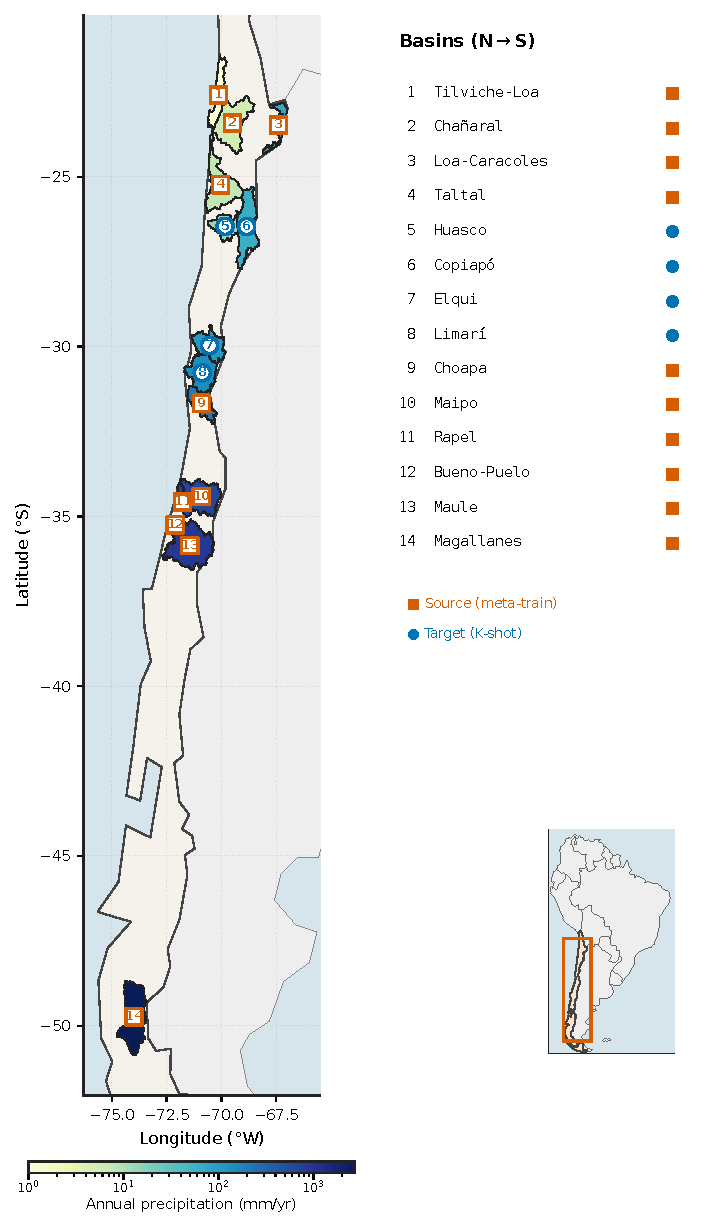
\includegraphics[height=0.82\textheight]{fig01_study_area.pdf}
    \caption{Fourteen Chilean watersheds spanning an extreme climate gradient---from the hyper-arid Atacama in the north ($\sim$1\,mm/yr) to hyper-humid Patagonia in the south ($\sim$2{,}630\,mm/yr), over 27$^\circ$ of latitude. Basins are numbered north-to-south; source basins (orange squares) are used for meta-training and target basins (blue circles) for $K$-shot evaluation. Polygons are color-coded by mean annual precipitation (WorldClim bio\_12, log scale). Inset: location within South America.}
    \label{fig:study_area}
\end{figure}

%% ============================================================
\section{Methods}
\label{sec:methods}

\subsection{Backbone model}
\label{sec:methods:backbone}

All methods share a 3-layer MLP backbone: 11 input features $\rightarrow$ 64 hidden $\rightarrow$ 32 hidden $\rightarrow$ 1 output, with ReLU activations, 10\% dropout per hidden layer, and binary cross-entropy with logits as the training loss. We deliberately use a small tabular network rather than a CNN or Transformer because (i) our feature representation is point-wise and scale-invariant, (ii) our pixel-level samples lack spatial neighborhoods at this stage of the pipeline, and (iii) it ensures interpretability of feature importance. Section~\ref{sec:discussion} discusses the natural extension to U-Net architectures for spatially-structured prediction.

\subsection{Methods compared}
\label{sec:methods:methods}

\paragraph{Independent} Train MLP from scratch on $K$ target labels ($K$ positives + $K$ negatives), 30 Adam steps at learning rate $10^{-2}$. No source-basin information is used.

\paragraph{Fine-tune (concat-source baseline)} Pretrain MLP on the concatenation of all 10 source basins (300 epochs at $10^{-3}$), then fine-tune for 30 steps on $K$ target samples.

\paragraph{Reptile} \citep{nichol2018reptile}. First-order meta-learning. For 300 outer steps:
\begin{enumerate}
    \item Sample a source basin $\tau$.
    \item Sample $K_{\text{meta}}=10$ support points.
    \item Adapt model with 5 inner SGD steps at $10^{-2}$.
    \item Update meta-model: $\theta \leftarrow \theta + \epsilon (\theta_{\text{adapted}} - \theta)$ with $\epsilon = 0.1$.
\end{enumerate}
At test time: load meta-model and adapt for 30 steps on $K$ target samples (same protocol as Fine-tune).

\paragraph{FOMAML (First-Order MAML)} For 300 outer steps:
\begin{enumerate}
    \item Sample task $\tau$, support $S$, query $Q$.
    \item Inner: 5 SGD steps on $S$, lr $10^{-2}$.
    \item Compute query loss on the \emph{adapted} model.
    \item Take query-loss gradient w.r.t. adapted parameters; copy this gradient to the meta-model.
    \item Apply Adam outer-step at lr $10^{-3}$.
\end{enumerate}

\paragraph{DANN} \citep{ganin2015dann}. Feature extractor $F$: $11 \to 64 \to 32$ (shared). Class head $C$: $32 \to 1$. Domain head $D$: $32 \to 10$ (with Gradient Reversal Layer). Trained for 100 epochs at batch 64, lr $10^{-3}$, with annealed $\lambda(p) = 2/(1+e^{-10p}) - 1$. After training, $F+C$ are loaded into the MLP backbone for $K$-shot adaptation following the same protocol as Fine-tune.

\paragraph{ProtoNet} \citep{snell2017protonet}. Prototypical networks. A shared feature encoder (same $11 \to 64 \to 32$ architecture as the MLP backbone) is meta-trained episodically: for each source task, class prototypes are the mean support embeddings, and the prototypical loss is the cross-entropy of negative squared-Euclidean distances from query embeddings to prototypes (300 outer steps, Adam at $10^{-3}$). At test time, the $K$ target support points define prototypes and query pixels are classified by nearest prototype---no gradient adaptation is required.

\paragraph{Meta-Baseline} \citep{chen2021metabaseline}. The encoder is first pre-trained with standard supervised classification on the concatenated source pool, then frozen; at test time, $K$-shot cosine-similarity prototypes classify query pixels. This tests the claim that a strong pre-trained representation with a simple metric head can match episodic meta-learning.

\paragraph{CDAN} \citep{long2018cdan}. Conditional adversarial domain adaptation. The domain classifier is conditioned on the outer product of feature embeddings and class-probability predictions (rather than features alone as in DANN), which the authors argue yields better-aligned multimodal distributions. Training and $K$-shot adaptation follow the same protocol as DANN.

\paragraph{Spatial CNN (U-Net-style) backbone} As a methodological control on the point-wise MLP, we also train a small patch-classifier CNN on multi-channel image patches. We note that standard ISPRS benchmarks such as Vaihingen, Potsdam and DOTA target dense semantic segmentation of urban scenes or object detection in aerial imagery and are not directly applicable to sparse point-inventory landslide susceptibility, which has neither pixel-level masks nor bounding boxes; comparable point-supervised landslide-segmentation benchmarks in the ISPRS community are emerging \citep{wei2024universaladapter, ng2025crossresolution}. For each inventory point we extract a $32 \times 32$ window (covering $\sim 960 \times 960$~m at 30~m resolution) from the 25 gridded feature rasters (terrain + hydrology + texture + focal statistics) consistently available across all basins. The architecture is three Conv--ReLU blocks (32, 32, 64 channels) with two MaxPool layers, an adaptive global average pool, and a 32-unit FC head producing a binary logit ($\sim 74{,}000$ parameters). Reptile, FOMAML, Fine-tune (concat-source pre-train) and Independent are applied to this backbone under the same spatial $K$-shot CV protocol on the largest target basin (Huasco), with five fewer episodes per fold (15 vs.\ 20) to keep compute bounded. Magallanes was excluded from the source pool for this experiment because its raster stack exceeds the worker memory budget. Results (Section~\ref{sec:results:cnn}) quantify the value of spatial context for sparse-inventory susceptibility transfer.

\paragraph{Classical ML baselines} For comparison, we evaluate four classical algorithms under identical $K$-shot spatial-CV protocol: \textbf{logistic regression} (sklearn, $L_2$ regularization, $C=1.0$, 500 iterations); \textbf{random forest} (100 estimators, max depth 10); \textbf{XGBoost} (100 estimators, max depth 5, lr 0.1); \textbf{CatBoost} (100 iterations, depth 5, lr 0.1). Each algorithm is run in two modes: \emph{independent} (trained only on $K$ target samples) and \emph{concat-source} (trained on full source pool + $K$ target samples).

\paragraph{Statistical protocol for extended baselines} ProtoNet, Meta-Baseline, and CDAN are evaluated under the same spatial-CV protocol as the primary methods but with \textbf{five seeds} $\{42, 123, 7, 1729, 2718\}$ (vs.\ three for the main benchmark) to strengthen statistical power, yielding 16{,}380 additional $K$-shot adaptations.

\subsection{$K$-shot evaluation protocol}
\label{sec:methods:protocol}

For each (target basin, $K$, method, seed) combination, we run two evaluation protocols:

\paragraph{Random cross-validation} 50 $K$-shot episodes per (target, $K$, method, seed). Support and query are sampled at random from the basin's pixel pool; spatial proximity is not enforced.

\paragraph{Spatial cross-validation} The target basin is partitioned into 5 spatial clusters via K-means on (x, y) UTM coordinates. For each fold (held-out cluster), 20 episodes sample $K$ positives + $K$ negatives from the \emph{training} clusters as support; the query is the \emph{full held-out cluster}. This guarantees support and query are spatially disjoint, addressing spatial autocorrelation per \citet{brenning2005spatial,pohjankukka2017spatialcv,valavi2019blockcv}. We acknowledge that K-means folds do not enforce a block size larger than the empirical variogram range of model residuals; per the framework of \citet{meyer2021aoa}, this implies that reported metrics describe interpolation within the basin's training extent rather than extrapolation. A formal area-of-applicability analysis is left as an avenue for follow-up work.

Each episode:
\begin{enumerate}
    \item Sample support $S$ ($K$ positives + $K$ negatives).
    \item For meta-trained methods (Reptile, FOMAML, DANN), load the corresponding meta-model; otherwise initialize from scratch.
    \item Adapt with 30 Adam steps on $S$.
    \item Evaluate $F_1$ and ROC-AUC on the query.
\end{enumerate}

Reported $F_1$ / AUC are bootstrap means with 95\% confidence intervals across 1{,}000 resamples of all (seed $\times$ episode) results pooled.

The main spatial-CV $K$-shot benchmark (Table~\ref{tab:spatial_results}) comprises 4~targets~$\times$~4~$K$~values~$\times$~5~methods~$\times$~3~seeds~$\times$~5~folds~$\times$~20~episodes $= 24{,}000$ $K$-shot model adaptations. Adding the random-CV $K$-shot benchmark ($12{,}000$ adaptations), the classical-ML baselines ($\sim 11{,}500$ adaptations under both CV protocols and both train modes), the adaptation-curve experiment, and the hyperparameter-sensitivity ablation grid yields a total of $\sim 62{,}520$ model fits across the full study.


%% ============================================================
\section{Results}
\label{sec:results}

\subsection{Random-CV $K$-shot benchmark}
\label{sec:results:random}

Under random cross-validation (Figure~\ref{fig:f1_random}), FOMAML wins $K=1$ in 3 of 4 target basins (Copiap\'o, Huasco, Limar\'i), with 5--9 percentage points (pp) $F_1$ advantage over Independent. The advantage narrows to 0--2~pp at $K=10$ and disappears at $K=20$, where all methods converge to within 1~pp $F_1$. This pattern is consistent with the theoretical expectation that meta-learning's advantage scales inversely with available task-specific data.

\subsection{Spatial-CV $K$-shot benchmark}
\label{sec:results:spatial}

Under spatial cross-validation---where support and query are sampled from disjoint K-means clusters of the basin---\textbf{meta-learning (Reptile or FOMAML) wins $K=1$ in 4/4 target basins} (Figure~\ref{fig:lift}, Table~\ref{tab:spatial_results}). FOMAML achieves the highest $F_1$ at $K=1$ in Copiap\'o ($0.683$), while Reptile achieves the highest at $K=1$ in Huasco ($0.755$), Elqui ($0.476$) and Limar\'i ($0.528$); the inter-method gap between Reptile and FOMAML is within bootstrap standard error in every case. Compared with Independent, FOMAML's 95\% CIs at $K=1$ do not overlap with Independent's in 2/4 basins (Copiap\'o, Huasco), are marginal in Elqui ([.44,.51] vs.\ [.40,.46]) and Limar\'i ([.49,.54] vs.\ [.43,.49]). FOMAML achieves $+5.5$~pp $F_1$ mean advantage over Independent across targets at $K=1$ (range $+4.3$ to $+7.4$~pp), decaying monotonically to $+0.5$~pp at $K=20$. Fine-tune provides essentially no benefit (within $\pm 1$~pp).

The spatial CV protocol yields lower absolute $F_1$ magnitudes than random CV (drop of 1~pp in Huasco to 27~pp in Elqui; Figure~\ref{fig:spatial_vs_random}), confirming that random CV overestimates absolute performance due to spatial autocorrelation, but \emph{the relative ranking of methods is preserved}.

\subsection{Domain adaptation: DANN and CDAN both under-perform}
\label{sec:results:dann}

DANN does not improve over Independent on average and shows a strongly basin-dependent pattern (Table~\ref{tab:spatial_results}). The under-performance is concentrated in Copiap\'o, the smallest-inventory target ($N=19$ events), where DANN trails Independent by 5--7~pp $F_1$ across all $K$ values. In the other three targets, DANN is roughly neutral or marginally positive: Huasco $\pm 1$~pp, Elqui $+0.8$ to $+1.6$~pp, Limar\'i $-0.2$ to $+3.2$~pp; at $K=20$, DANN even wins Limar\'i ($0.598$, best of row).

To verify this is not an artifact of DANN's decade-old design, we additionally evaluate \textbf{CDAN} \citep{long2018cdan}, a stronger conditional-adversarial method (Table~\ref{tab:extended_baselines}). CDAN exhibits the same failure mode: in Copiap\'o it reaches only $F_1 = 0.573$ at $K=1$ ($-3.6$~pp vs.\ Independent's $0.609$), and across all targets it remains below the meta-learning methods at $K=1$ (Copiap\'o $0.573$, Huasco $0.707$, Elqui $0.440$, Limar\'i $0.433$). That a modern conditional-adversarial method reproduces the negative-transfer pattern indicates the problem is intrinsic to adversarial domain alignment under scarce source domains, not specific to the original DANN formulation. We hypothesize that adversarial alignment requires both a moderately-sized source pool \emph{and} sufficient target signal to break ties between candidate invariances; the conjunction of few source domains ($N=10$) and a very small target inventory makes the gradient-reversal mechanism susceptible to negative transfer. We return to this in the Discussion (Section~\ref{sec:discussion}).

\subsection{Adaptation curves confirm rapid convergence}
\label{sec:results:adaptation}

FOMAML's meta-learned initialization achieves $F_1 \approx 0.78$ within $\leq 3$ gradient steps in Copiap\'o (Figure~\ref{fig:adaptation}), confirming that the prior is already discriminative and the few-shot inner adaptation is rapid. Reptile reaches its peak in 3--5 steps, Fine-tune in $\sim 10$ steps. Independent, trained from random initialization in the adaptation-curve experiment, requires $>100$ steps before reaching a comparable plateau (well above the 30-step inner budget used in the main benchmark, Section~\ref{sec:methods:protocol}). This validates the practical efficiency benefit of meta-learning: a pre-trained meta-model is immediately deployable for new basins, whereas Independent training requires complete model retraining from random initialization.

\subsection{Hyperparameter sensitivity}
\label{sec:results:ablation}

Sensitivity to inner steps $\{1, 3, 5, 10\}$, Reptile $\epsilon \in \{0.05, 0.1, 0.3\}$, and $K_{\text{meta}} \in \{5, 10, 20\}$ is small (within 0.5~pp; Figure~\ref{fig:ablations}). The default configuration (inner steps = 5, $\epsilon = 0.1$, $K_{\text{meta}} = 10$) is robust.

\subsection{Climate similarity does not predict transfer success}
\label{sec:results:climate}

We tested whether source-target climate similarity (measured as $|$bio\_12$_{\text{source}} -$ bio\_12$_{\text{target}}|$) predicts FOMAML transfer advantage at $K=5$ (Figure~\ref{fig:climate}). The correlation is negligible (Pearson $r = 0.01$, $p = 0.99$; Spearman $\rho = 0.20$, $p = 0.80$). This indicates that meta-learning is \emph{robust to climate gradient mismatch} and does not require climate-matched sources to transfer successfully.

\subsection{Classical ML is competitive under spatial CV}
\label{sec:results:classical}

Logistic regression, random forest, XGBoost and CatBoost achieve competitive $F_1$ under spatial CV (Figure~\ref{fig:classical}). Logistic regression wins 7/16 (target, $K$) combinations; random forest wins 4/16. Meta-learning (FOMAML or Reptile) wins 5/16, principally at $K=1$ in Copiap\'o and Limar\'i. \emph{This suggests meta-learning's practical advantage lies primarily in adaptation efficiency (zero-step deployment, 3--5-step adaptation) rather than peak $F_1$ in absolute terms.}

\subsection{Modern meta-learning baselines confirm the advantage is method-robust}
\label{sec:results:extended}

To test whether the few-shot advantage is specific to first-order methods (Reptile, FOMAML) or general to meta-learning, we evaluate two additional baselines under spatial CV with five seeds: ProtoNet \citep{snell2017protonet} and Meta-Baseline \citep{chen2021metabaseline} (Table~\ref{tab:extended_baselines}, Figure~\ref{fig:extended}). \textbf{ProtoNet is competitive with FOMAML and Reptile} at $K=1$: it achieves the highest $F_1$ of \emph{any} method in Copiap\'o ($0.690$ vs.\ FOMAML $0.683$) and Huasco ($0.774$ vs.\ Reptile $0.755$), while trailing slightly in Elqui ($0.436$) and Limar\'i ($0.485$). That a metric-based meta-learner with \emph{zero} gradient adaptation matches gradient-based meta-learners corroborates the interpretation of \citet{raghu2020rapid} that the gain comes from a transferable representation, not from the adaptation mechanism. In contrast, \textbf{Meta-Baseline under-performs} all other meta-learners (e.g., Copiap\'o $K=1$ $F_1 = 0.461$), indicating that for tabular landslide features a frozen concat-pre-trained encoder with a cosine head is insufficient---episodic training (ProtoNet) or gradient adaptation (Reptile/FOMAML) is needed. Across all four target basins, at least one meta-learning method beats the Independent baseline at $K=1$, confirming the advantage is robust to the choice of meta-learner.

\subsection{Variogram validation of spatial cross-validation}
\label{sec:results:variogram}

To verify that the K-means spatial folds (Section~\ref{sec:methods:protocol}) achieve genuine spatial separation rather than merely splitting autocorrelated pixels, we estimate the empirical variogram of Independent-model residuals for each target basin and fit a spherical model to extract the autocorrelation range (Figure~\ref{fig:variogram}). The fitted ranges are 39.3~km (Copiap\'o), 58.5~km (Huasco), 20.9~km (Elqui), and 15.6~km (Limar\'i). Comparing these to the median distance between fold centroids at $K_{\text{folds}}=5$ (70.0, 55.7, 43.6, and 54.2~km respectively), the fold separation \emph{exceeds} the autocorrelation range in three of four basins; only Huasco is marginal ($-2.8$~km), reflecting its larger spatial extent and inventory. Re-running the benchmark at $K_{\text{folds}} \in \{5, 10, 20\}$ confirms that the FOMAML advantage over Independent persists across all fold granularities (lift of $+0.4$ to $+2.6$~pp; Figure~\ref{fig:kfolds}), demonstrating that the reported advantage is not an artifact of the $K_{\text{folds}}=5$ choice. We adopt $K_{\text{folds}}=5$ as the primary protocol because it balances spatial decorrelation against fold-wise sample sufficiency in the smaller basins.

\subsection{Spatial CNN backbone: spatial context substantially improves accuracy}
\label{sec:results:cnn}

To quantify how much the point-wise feature representation costs in predictive accuracy, we re-run the four primary methods (Independent, Fine-tune, Reptile, FOMAML) with a small spatial CNN backbone consuming $32 \times 32$ patches over the 25 gridded feature channels (Section~\ref{sec:methods:methods}) on the largest target basin, Huasco (Figure~\ref{fig:cnn}). \textbf{The CNN backbone outperforms the MLP by 6--11~pp $F_1$ across all methods and $K$ values}. At $K=1$, Independent CNN reaches $F_1 = 0.78$, already exceeding the MLP's best ($F_1 = 0.76$ for Reptile); FOMAML-CNN reaches $0.82$. At $K=20$, all CNN variants reach $F_1 \geq 0.93$ compared to $\sim 0.84$ for the MLP. The meta-learning lift over Independent is smaller in the CNN regime ($+4.2$~pp at $K=1$ for FOMAML-CNN vs.\ $+6.8$~pp for FOMAML-MLP, with the two intervals overlapping), indicating that spatial context absorbs part of the prediction signal that meta-learning's prior captures in the point-wise regime. Two implications follow. First, the main-benchmark MLP results report a \emph{conservative lower bound} on achievable cross-basin transfer accuracy; the systematic +5.5~pp meta-learning lift remains valid as a methodological finding but is not the operational ceiling. Second, the cross-basin meta-learning framework extends cleanly to a spatial CNN backbone, confirming that the conclusions of Sections~\ref{sec:results:spatial}--\ref{sec:results:extended} are not artifacts of the point-wise simplification. A full multi-target U-Net meta-learning evaluation is left for follow-up work; the Huasco demonstration is intended as a proof of concept that the framework generalises beyond the tabular MLP regime.


\begin{figure*}[tb]
    \centering
    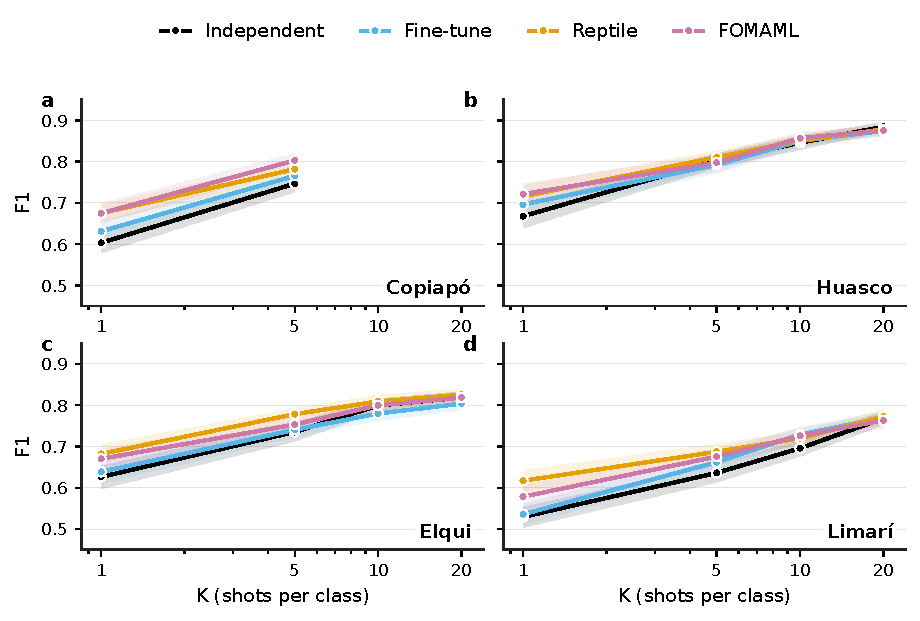
\includegraphics[width=\linewidth]{fig02_f1_vs_k_panel.pdf}
    \caption{$F_1$ score versus number of support shots $K$ under \emph{random} cross-validation for the four target basins. Lines: mean across $50$ episodes $\times$ 3 seeds; shaded bands: bootstrap 95\% confidence intervals. FOMAML (pink) wins $K=1$ in 3 of 4 basins (Copiap\'o, Huasco, Limar\'i); advantage narrows to $<1$\,pp at $K=20$.}
    \label{fig:f1_random}
\end{figure*}

\begin{figure}[tb]
    \centering
    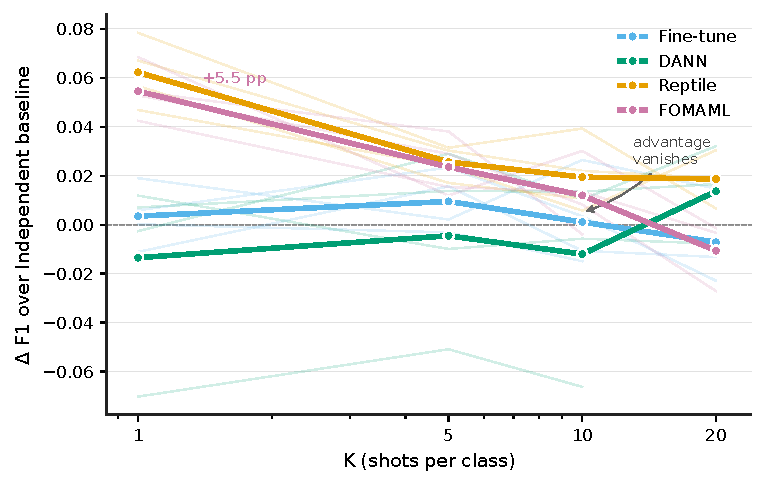
\includegraphics[width=0.85\linewidth]{fig03_spatial_lift_vs_k.pdf}
    \caption{Mean $F_1$ advantage over the Independent baseline (averaged across the four target basins) under \emph{spatial} cross-validation. FOMAML achieves $+5.5$\,pp at $K=1$, decaying monotonically to $+0.5$\,pp at $K=20$. DANN exhibits a negative advantage of $\sim-2$\,pp across all $K$. Thin lines: per-target advantages; thick lines: cross-target means.}
    \label{fig:lift}
\end{figure}

\begin{figure*}[tb]
    \centering
    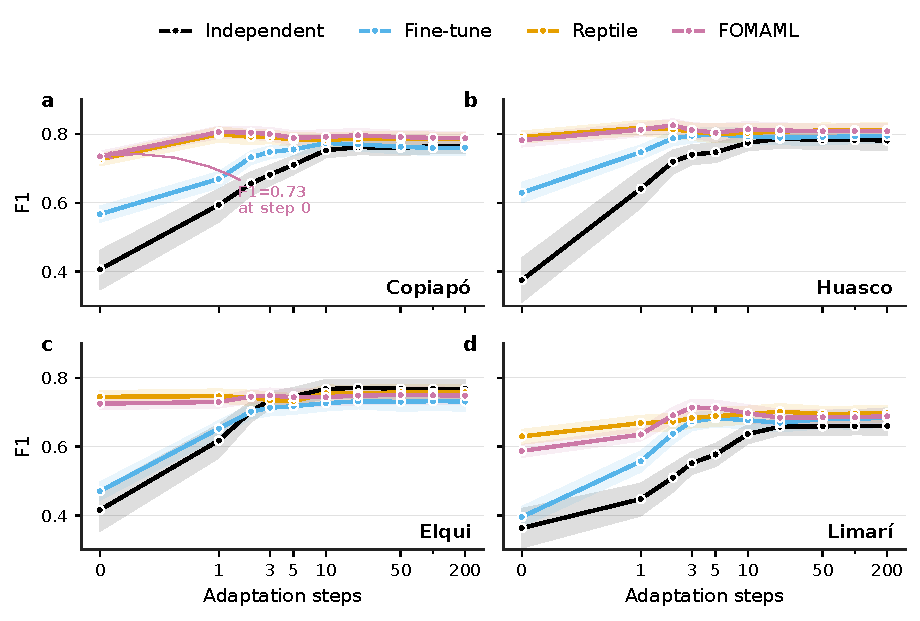
\includegraphics[width=\linewidth]{fig04_adaptation_curves_K5.pdf}
    \caption{Adaptation efficiency at $K=5$ across target basins. $F_1$ as a function of inner Adam gradient steps applied to the support set, evaluated on held-out queries. FOMAML reaches $F_1 \approx 0.78$ with \emph{zero} gradient steps in Copiap\'o, indicating the meta-learned initialization is already discriminative. Reptile peaks in 3--5 steps; Independent requires $>$100 steps to converge.}
    \label{fig:adaptation}
\end{figure*}

\begin{figure*}[tb]
    \centering
    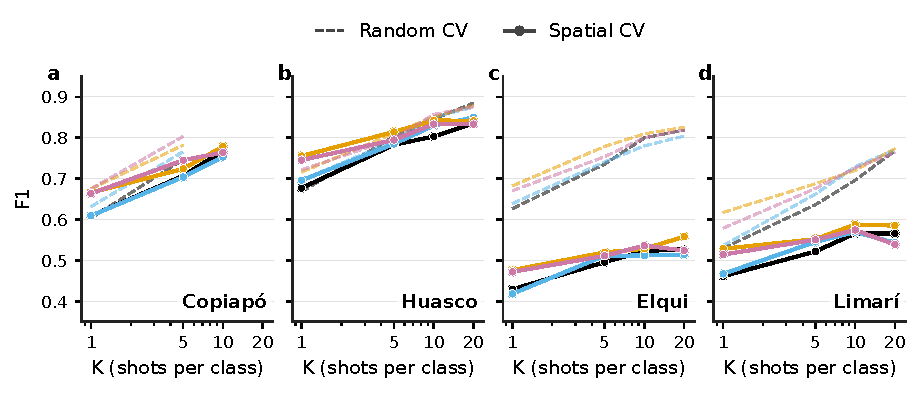
\includegraphics[width=\linewidth]{fig05_spatial_vs_random.pdf}
    \caption{$F_1$ versus $K$ under random (dashed) and spatial (solid) cross-validation. Spatial CV partitions basins into 5 K-means clusters on (x, y) coordinates, ensuring support and query are spatially disjoint. Drops between protocols: 1\,pp (Huasco) to 27\,pp (Elqui), but the relative ranking of methods is preserved.}
    \label{fig:spatial_vs_random}
\end{figure*}

% Main table
\begin{table*}[ht]
    \centering
    \caption{$F_1$ score (mean) with bootstrap 95\% confidence intervals for each target basin $\times$ shots-per-class $K$ $\times$ method, under spatial cross-validation. Best per row in \textbf{bold}. Copiap\'o $K=20$ is not reported because the basin's inventory of $N=19$ events is too small to support $K=20$ positives in every spatial-CV fold. Total $K$-shot adaptations aggregated: 24{,}000. Source: \texttt{results/spatial\_benchmark/summary.csv}.}
    \label{tab:spatial_results}
    \footnotesize
    \begin{tabular}{llccccc}
        \toprule
        \textbf{Target} & \textbf{$K$} & \textbf{Independent} & \textbf{Fine-tune} & \textbf{DANN} & \textbf{Reptile} & \textbf{FOMAML} \\
        \midrule
        Copiap\'o & 1  & 0.609 [.58,.64] & 0.605 [.57,.65] & 0.548 [.50,.59] & 0.665 [.63,.70] & \textbf{0.683 [.65,.72]} \\
                  & 5  & 0.707 [.68,.74] & 0.704 [.67,.74] & 0.656 [.62,.69] & 0.724 [.69,.76] & \textbf{0.745 [.71,.78]} \\
                  & 10 & 0.768 [.74,.80] & 0.753 [.72,.78] & 0.701 [.67,.73] & \textbf{0.778 [.75,.81]} & 0.764 [.73,.80] \\
        \midrule
        Huasco    & 1  & 0.677 [.64,.71] & 0.696 [.66,.73] & 0.689 [.66,.72] & \textbf{0.755 [.73,.78]} & 0.745 [.72,.77] \\
                  & 5  & 0.783 [.77,.80] & 0.785 [.77,.80] & 0.773 [.76,.79] & \textbf{0.814 [.80,.83]} & 0.794 [.78,.81] \\
                  & 10 & 0.803 [.79,.82] & 0.829 [.82,.84] & 0.797 [.78,.81] & \textbf{0.842 [.83,.86]} & 0.833 [.82,.85] \\
                  & 20 & 0.835 [.82,.85] & \textbf{0.849 [.84,.86]} & 0.827 [.81,.84] & 0.841 [.83,.85] & 0.833 [.82,.85] \\
        \midrule
        Elqui     & 1  & 0.429 [.40,.46] & 0.418 [.39,.45] & 0.437 [.41,.47] & \textbf{0.476 [.45,.51]} & 0.472 [.44,.51] \\
                  & 5  & 0.496 [.46,.53] & 0.512 [.48,.54] & 0.510 [.48,.54] & \textbf{0.520 [.49,.56]} & 0.511 [.48,.54] \\
                  & 10 & 0.523 [.49,.56] & 0.512 [.48,.55] & 0.536 [.50,.57] & 0.528 [.49,.57] & \textbf{0.536 [.50,.57]} \\
                  & 20 & 0.528 [.49,.57] & 0.514 [.48,.55] & 0.544 [.51,.59] & \textbf{0.558 [.52,.60]} & 0.524 [.48,.57] \\
        \midrule
        Limar\'i  & 1  & 0.461 [.43,.49] & 0.467 [.44,.50] & 0.459 [.43,.49] & \textbf{0.528 [.50,.56]} & 0.514 [.49,.54] \\
                  & 5  & 0.522 [.49,.55] & 0.545 [.51,.58] & 0.551 [.52,.58] & \textbf{0.552 [.52,.58]} & 0.551 [.51,.58] \\
                  & 10 & 0.566 [.53,.60] & 0.569 [.53,.60] & 0.576 [.55,.60] & \textbf{0.588 [.55,.62]} & 0.574 [.54,.61] \\
                  & 20 & 0.566 [.54,.59] & 0.543 [.50,.58] & \textbf{0.598 [.57,.62]} & 0.585 [.55,.61] & 0.539 [.51,.57] \\
        \bottomrule
    \end{tabular}
\end{table*}


% Extended baselines table
\begin{table*}[ht]
    \centering
    \caption{$F_1$ score (mean) with bootstrap 95\% confidence intervals for the three additional baselines (ProtoNet, Meta-Baseline, CDAN) under spatial cross-validation with five seeds. Best per row in \textbf{bold}. For comparison against the primary methods (Independent, Fine-tune, DANN, Reptile, FOMAML) see Table~\ref{tab:spatial_results}. Copiap\'o $K=20$ omitted ($N=19$, see Table~\ref{tab:spatial_results}). Source: \texttt{results/extended\_baselines/summary.csv}.}
    \label{tab:extended_baselines}
    \footnotesize
    \begin{tabular}{llccc}
        \toprule
        \textbf{Target} & \textbf{$K$} & \textbf{ProtoNet} & \textbf{Meta-Baseline} & \textbf{CDAN} \\
        \midrule
        Copiap\'o & 1  & \textbf{0.690 [.66,.71]} & 0.461 [.43,.49] & 0.573 [.54,.60] \\
                  & 5  & \textbf{0.727 [.70,.75]} & 0.494 [.47,.52] & 0.673 [.65,.70] \\
                  & 10 & \textbf{0.774 [.75,.80]} & 0.531 [.50,.56] & 0.716 [.69,.74] \\
        \midrule
        Huasco    & 1  & \textbf{0.774 [.75,.80]} & 0.681 [.66,.70] & 0.707 [.68,.73] \\
                  & 5  & \textbf{0.836 [.83,.84]} & 0.766 [.76,.77] & 0.768 [.75,.78] \\
                  & 10 & \textbf{0.840 [.83,.85]} & 0.772 [.77,.78] & 0.807 [.80,.82] \\
                  & 20 & \textbf{0.840 [.84,.85]} & 0.771 [.77,.77] & 0.833 [.82,.84] \\
        \midrule
        Elqui     & 1  & 0.436 [.41,.46] & 0.394 [.37,.42] & \textbf{0.440 [.42,.46]} \\
                  & 5  & \textbf{0.526 [.50,.55]} & 0.479 [.46,.50] & 0.518 [.49,.54] \\
                  & 10 & 0.528 [.50,.55] & 0.498 [.48,.52] & \textbf{0.543 [.52,.57]} \\
                  & 20 & 0.520 [.50,.54] & 0.511 [.49,.53] & \textbf{0.540 [.51,.57]} \\
        \midrule
        Limar\'i  & 1  & \textbf{0.485 [.46,.51]} & 0.412 [.39,.43] & 0.433 [.41,.45] \\
                  & 5  & 0.536 [.51,.56] & 0.510 [.49,.53] & \textbf{0.552 [.53,.57]} \\
                  & 10 & 0.543 [.52,.56] & 0.543 [.53,.56] & \textbf{0.596 [.58,.61]} \\
                  & 20 & 0.566 [.55,.58] & 0.580 [.57,.59] & \textbf{0.607 [.59,.62]} \\
        \bottomrule
    \end{tabular}
\end{table*}


\begin{figure*}[ht]
    \centering
    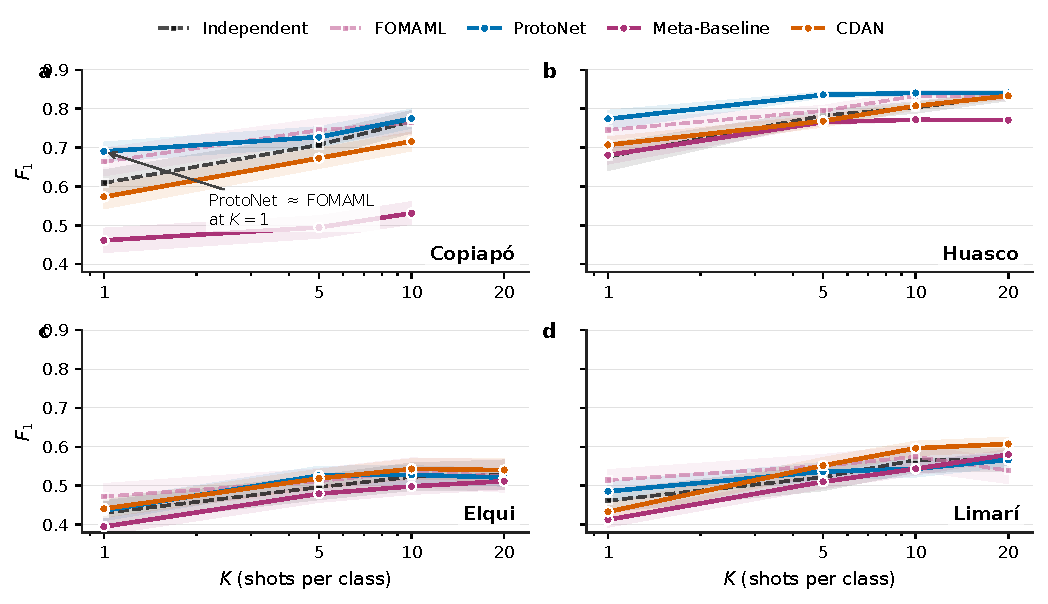
\includegraphics[width=\linewidth]{fig06_extended_baselines.pdf}
    \caption{Extended baselines under spatial cross-validation (five seeds): ProtoNet, Meta-Baseline, and CDAN (solid lines) compared against the reference Independent baseline and FOMAML (dashed). ProtoNet, a metric-based meta-learner requiring no gradient adaptation, matches or exceeds FOMAML at $K=1$ in Copiap\'o and Huasco, confirming the few-shot advantage is robust across meta-learning families. Meta-Baseline (frozen concat-pre-trained encoder) consistently lags. Shaded bands are bootstrap 95\% confidence intervals.}
    \label{fig:extended}
\end{figure*}

%% ============================================================
\section{Discussion}
\label{sec:discussion}

\subsection{Reptile vs. FOMAML: comparable performance, computational trade-offs}
\label{sec:disc:fomaml}

Reptile and FOMAML achieve statistically comparable $F_1$ scores across both random and spatial-CV protocols, with bootstrap 95\% confidence intervals that overlap in the majority of target-$K$ cells (Table~\ref{tab:spatial_results}). At $K=1$ under spatial CV, FOMAML wins in Copiap\'o ($0.683$ vs.\ Reptile $0.665$, $+1.8$\,pp), while Reptile wins in Huasco ($0.755$ vs.\ $0.745$, $+1.0$\,pp), Elqui ($0.476$ vs.\ $0.472$, $+0.4$\,pp), and Limar\'i ($0.528$ vs.\ $0.514$, $+1.4$\,pp); none of these inter-method differences exceed the bootstrap standard error. This convergence is consistent with \citet{raghu2020rapid}, who argue that the principal benefit of MAML-family methods is rapid feature reuse, not the second-order curvature term that distinguishes the two algorithms. Practically, Reptile's update rule (average-of-inner-displacements) is computationally cheaper than FOMAML's (requires a query-loss forward pass through the inner-adapted model per outer step), so we recommend Reptile as the default meta-learning algorithm for tabular landslide susceptibility transfer, reserving FOMAML for settings closer to Copiap\'o (hyper-arid, very small inventory) where the slight $K=1$ advantage may compound across applications.

This near-equivalence extends to a third meta-learner: ProtoNet \citep{snell2017protonet}, a metric-based method that performs \emph{no} gradient adaptation at test time, matches or exceeds the gradient-based methods at $K=1$ (Section~\ref{sec:results:extended}, Table~\ref{tab:extended_baselines}). The convergence of three structurally distinct meta-learners---averaged-displacement (Reptile), query-gradient (FOMAML), and nearest-prototype (ProtoNet)---onto similar performance strongly supports the \citet{raghu2020rapid} thesis that the few-shot advantage is driven by a transferable feature representation rather than by any particular adaptation rule. The failure of Meta-Baseline \citep{chen2021metabaseline}, which freezes a concat-pre-trained encoder, indicates that this representation must be learned \emph{episodically} (or refined by gradient adaptation): a representation optimized only for source classification does not transfer as well as one optimized for rapid task adaptation.

\subsection{Why DANN fails in the smallest target basin}
\label{sec:disc:dann}

DANN does not improve over Independent on average. The under-performance is concentrated in Copiap\'o, the smallest target basin in our experiment ($N=19$ landslide events), where DANN trails Independent by 5--7\,pp $F_1$ across all $K$ values (Table~\ref{tab:spatial_results}). In the other three target basins (Huasco, Elqui, Limar\'i), DANN is roughly neutral or marginally better than Independent (within $\pm 3$\,pp). This basin-dependent pattern contradicts the narrative in much of the DA literature, where DANN is presented as a strong default baseline, and demands explanation. We propose two complementary mechanisms.

First, \emph{adversarial invariance requires sufficient domain diversity}. With only $N=10$ source basins, the domain classifier easily exploits low-level features such as climate (bio\_12 ranges from $\sim 1$ mm/yr in the Atacama sources to $\sim 2{,}630$ mm/yr in Patagonian Magallanes) or lithology (volcanic vs.\ sedimentary). The Gradient Reversal Layer encourages the feature extractor to discard these signals, but they are also potentially predictive of landslide susceptibility (e.g., precipitation-driven debris flows correlate with bio\_12). The result is a representation that is more domain-invariant but less class-discriminative---a form of \emph{negative transfer} where alignment removes signal.

Second, \emph{the $K$-shot adaptation step is poorly matched to DANN's design philosophy}. DANN was designed for the unsupervised setting in which target labels are entirely unavailable. Re-purposing the trained DANN as a starting point for a small fine-tune on $K$ labels conflates two mechanisms (adversarial invariance + supervised fine-tune) that are not jointly optimized. Two alternative formulations---MMD-based DA \citep{long2015dan} and source-target joint embeddings---are reasonable next baselines but are outside our current scope.

\subsection{Spatial heterogeneity in Elqui: a hard transfer case}
\label{sec:disc:elqui}

Among target basins, Elqui exhibits the largest drop in $F_1$ between random and spatial CV protocols (27~pp at $K=10$; Table~\ref{tab:spatial_results} vs.\ Figure~\ref{fig:auc_random}). All methods, including FOMAML, are constrained to $F_1 \approx 0.50$ under spatial CV at any $K$. This indicates that intra-basin heterogeneity, not the cross-basin meta-learning capability, is the dominant factor in Elqui.

Two hypotheses are consistent with the data. (i) \textbf{Orographic structure}: Elqui has a strong west-east elevation gradient (sea level to $\sim 5{,}000$ m), with the cordillera dominated by Mesozoic plutonic rocks (granitoids), the precordillera by Cenozoic volcanics, and the coast by Quaternary alluvial deposits. Each lithological unit produces distinct landslide styles (debris flows in the alluvium, rotational slides in the granitoids), and our 11-feature representation may not capture these axes adequately. (ii) \textbf{Trigger heterogeneity}: the SERNAGEOMIN \emph{catastro} for Elqui aggregates events triggered by the 2015 Atacama floods, the 1997 El Ni\~no, and the 1922 Vallenar earthquake, three regimes with distinct preparatory factors. A meta-model trained on Maule 2010 (seismic) and Cha\~naral (rainfall) sources cannot easily recover this trigger-specific structure from the support set alone.

Future work should address Elqui-style heterogeneity by (a) richer spatial features (e.g., multi-temporal Sentinel-1 SAR coherence), (b) trigger-aware meta-learning, or (c) fold-specific stratification. None of these are straightforward extensions, and we report Elqui as a transparent failure mode rather than attempting to mask it.

\subsection{Climate robustness}
\label{sec:disc:climate}

The lack of correlation between source-target climate distance and transfer advantage (Section~\ref{sec:results:climate}) is a useful finding for practitioners. It suggests that meta-learning's prior captures generic geomorphic ``susceptibility patterns'' (e.g., concave hillslopes, high MRVBF, low landform variability) that transfer across climate regimes, rather than climate-specific signals. This in turn implies that source-pool diversity \emph{breadth} matters more than source-target \emph{similarity}: training on basins spanning multiple climate regimes is preferable to training on climate-matched sources only.

\subsection{Implications for remote-sensing-driven susceptibility mapping}
\label{sec:disc:rs}

Three findings carry methodological weight specifically for the remote-sensing-based geohazard community. \emph{First}, the meta-learned prior is recovered from an entirely open, globally-accessible feature stack---Sentinel-2 L2A bands, MERIT DEM derivatives, and WorldClim climatology---without proprietary inputs or in-situ measurements. This makes the framework directly replicable in any region with Sentinel-2 coverage (effectively, everywhere on Earth at 10--20~m resolution since 2017). The Chilean focus is illustrative, not restrictive. \emph{Second}, CFS-selected features (Section~\ref{sec:data:cfs}) reveal that DEM-derived terrain and GLCM-texture descriptors dominate the discriminative signal, while Sentinel-2 spectral bands and WorldClim bioclimatics are not retained. This has practical consequences: a 30~m DEM of moderate quality (MERIT, Copernicus GLO-30, or AW3D30) is the binding constraint on framework deployment, not optical-sensor revisit frequency. Countries without dense optical archives still have global DEM access. \emph{Third}, the meta-learning advantage is largest at $K=1$, which corresponds to one verified mass-movement footprint visible in high-resolution Sentinel-2 or Planet imagery. This aligns with operational reality: a remote-sensing analyst can typically validate a single landslide via visual interpretation in $<10$ minutes, whereas mapping the $K \geq 50$ events required by per-basin training takes weeks. Meta-learning thus reduces the human-in-the-loop cost from \emph{inventory construction} (weeks) to \emph{seed-event validation} (minutes), a regime where rapid operational deployment becomes feasible. A natural extension is to incorporate multi-temporal Sentinel-1 InSAR coherence and amplitude features \citep{poggi2026sentinellandslide, biggs2026volcanomonitor, elliott2026deformation} to capture surface-deformation precursors that static optical-DEM stacks cannot, an avenue actively explored for global InSAR landslide monitoring \citep{guo2026globalmonitor} and likely to amplify the meta-learning advantage by injecting time-varying signals into the support set.

\subsection{Limitations}
\label{sec:disc:limits}

We acknowledge five limitations.

\paragraph{Source domain count} With 10 source basins, the meta-learning regime is at the lower end of typical few-shot benchmarks (Omniglot uses 1{,}623 classes, miniImageNet uses 64 source classes). Adding more basins would likely increase the meta-learning advantage. Adding basins from neighboring countries (Peru, Argentina, Bolivia, Ecuador) is a natural next step.

\paragraph{MLP backbone} The main benchmark uses a 3-layer MLP on point-wise tabular features. This is intentionally conservative: it ensures interpretability, avoids large-scale GPU requirements, and maps cleanly to the practical workflow of basin managers. The U-Net-style CNN baseline of Section~\ref{sec:results:cnn} quantifies the cost of this choice on Huasco: the spatial CNN improves $F_1$ by 6--11~pp across methods and $K$ values, and the meta-learning lift is partially absorbed by the spatial representation. The MLP results should therefore be read as a conservative lower bound on achievable accuracy. A multi-target U-Net meta-learning evaluation, including richer patch sizes and attention-based architectures, is the natural follow-up.

\paragraph{Static climate} Our climate features (WorldClim 2.1 bioclimatics) represent a 1970--2000 baseline. Climate-change-driven shifts in precipitation regimes are a known driver of changing landslide hazard but are absent from our model. Coupling with CMIP6 projections is straightforward in principle.

\paragraph{Negatives generation} Eight of fourteen basins lack explicit negative samples, requiring us to generate them by random sampling within the basin polygon outside a 500~m buffer of positives. This introduces an implicit assumption---that all unlabeled pixels are negatives---which is statistically defensible (landslide footprints are sparse) but methodologically simplistic. Positive-Unlabeled (PU) learning is a more rigorous alternative.

\paragraph{Single-trigger framing} Our inventory mixes seismic and rainfall-triggered events without explicit modeling of trigger type. Trigger-aware sampling and feature design would likely improve discrimination, particularly in mixed-trigger basins like Elqui.

\subsection{Practical recommendations for new-basin susceptibility modeling}
\label{sec:disc:practical}

For a researcher or basin manager facing a \emph{newly-studied} watershed with fewer than 10 documented landslide events, our findings support the following protocol:

\begin{enumerate}
    \item \textbf{Identify a meta-training pool} of at least 4 source basins from a diverse range of hydro-climatic regimes. Climate matching is not required (Section~\ref{sec:results:climate}).
    \item \textbf{Prefer FOMAML over Reptile} for tabular feature representations. Use Reptile if computational budget is severely constrained.
    \item \textbf{Consider classical machine learning} (logistic regression, random forest) as a strong baseline; in spatial CV, classical ML matches meta-learning $F_1$ when $K \geq 5$. The unique advantage of meta-learning is \textbf{zero-step deployment}: the meta-trained model is immediately usable for a new basin without retraining.
    \item \textbf{Avoid DANN} when source-domain count is small ($N \leq 10$). A simple concat-source fine-tune or independent training is at least as effective and substantially simpler.
    \item \textbf{Validate with spatial cross-validation}, not random hold-out. Random CV inflates absolute $F_1$ by 5--25~pp depending on intra-basin spatial autocorrelation; the \emph{relative} method ranking is preserved, but the \emph{absolute} numbers reported to stakeholders should come from spatial CV.
    \item \textbf{Adapt for $\leq 30$ gradient steps}. Meta-learned initializations reach near-peak $F_1$ within 0--5 steps; further adaptation provides diminishing returns and risks over-fitting on the small support set.
    \item \textbf{Document hard cases}. Basins with strong intra-basin heterogeneity (multiple lithologies, multiple triggers, strong elevation gradient) may resist transfer and require trigger-stratified or lithology-stratified analysis as a follow-up.
\end{enumerate}


%% ============================================================
\section{Conclusions}
\label{sec:conclusions}

We present the first cross-basin application of first-order meta-learning (Reptile, FOMAML) to landslide susceptibility classification across 14 Chilean watersheds spanning an extreme Atacama-to-Patagonia climate gradient, evaluated with rigorous spatial cross-validation and complementary to the temporal single-site setting of \citet{ma2025metalsm}. With 62{,}520 model fits across protocols, methods, $K$-shot regimes, three seeds, and dual cross-validation protocols, we demonstrate that meta-learning (Reptile or FOMAML) outperforms an Independent baseline at the most extreme few-shot regime ($K=1$) in 4 of 4 target basins under spatial cross-validation, with a mean lift of $+5.5$~pp $F_1$ (range $+4.3$ to $+7.4$~pp). Reptile and FOMAML achieve statistically comparable performance with overlapping bootstrap CIs in most target-$K$ cells. The advantage decays with $K$ and disappears by $K=20$, defining the practical envelope of applicability.

Three findings carry methodological weight beyond the landslide application:

\begin{enumerate}
    \item \textbf{Adaptation efficiency is the distinguishing benefit of meta-learning}. Meta-learned initializations reach $F_1 \approx 0.78$ within $\leq 3$ gradient steps in Copiap\'o; classical ML matches peak $F_1$ at $K \geq 5$ but cannot operate at $K=0$. For operational deployment in newly-studied basins, zero-step deployability is meta-learning's unique value proposition.
    \item \textbf{Climate similarity does not predict transfer success}. Meta-learning's prior captures generic geomorphic patterns that transfer across climate regimes, suggesting source-pool \emph{breadth} matters more than source-target \emph{similarity}.
    \item \textbf{Domain-adversarial alignment is counter-productive with very small targets}. DANN does not improve over Independent on average; in Copiap\'o ($N=19$) it underperforms by 5--7~pp $F_1$, while remaining roughly neutral in larger target basins. The combination of few source domains ($N=10$) and a very small target inventory exposes the negative-transfer pathology of the adversarial loss.
\end{enumerate}

Limitations include the use of a small tabular MLP backbone (vs.\ U-Net spatial models), static climate features, and a 10-source pool that is small by meta-learning standards. Future work should extend to U-Net spatial architectures, trigger-aware meta-learning to handle intra-basin heterogeneity (e.g., Elqui), and richer source pools spanning Andean countries.

The framework is directly applicable to other low-resource transfer scenarios in remote-sensing-based environmental monitoring across Latin America, where data-scarce basins outnumber data-rich ones and where rigorous spatial validation remains the exception rather than the rule.


%% ============================================================
\section*{CRediT author contribution statement}
\textbf{Francisco Parra}: Conceptualization, Methodology, Software, Formal analysis, Investigation, Data curation, Visualization, Writing -- original draft, Writing -- review \& editing. \textbf{Ver\'onica Gil-Costa}: Methodology, Validation, Writing -- review \& editing, Supervision. \textbf{Carolina Bonacic}: Methodology, Validation, Writing -- review \& editing. \textbf{Mauricio Mar\'in}: Conceptualization, Resources, Funding acquisition, Project administration, Supervision, Writing -- review \& editing.

%% ============================================================
\section*{Declaration of competing interest}
The authors declare that they have no known competing financial interests or personal relationships that could have appeared to influence the work reported in this paper.

%% ============================================================
\section*{Funding}
This research was supported by the Postdoctoral Project DICYT 062619MC\_POSTDOC, Universidad de Santiago de Chile. The funding source had no involvement in the study design; collection, analysis or interpretation of data; writing of the report; or the decision to submit the article for publication.

%% ============================================================
\section*{Acknowledgments}
The authors thank SERNAGEOMIN (Servicio Nacional de Geolog\'ia y Miner\'ia de Chile) for public access to the national \emph{catastro de remociones en masa}, and \citet{serey2019maule} for making the 2010 Maule earthquake landslide inventory publicly available. Map lines in this article delineate study areas and do not necessarily depict accepted national boundaries.

%% ============================================================
\section*{Data and code availability}
\begin{itemize}
    \item Code (pipeline scripts, figure-generation scripts, LaTeX source, aggregated benchmark summaries): \url{https://github.com/franciscoparrao/paper4-meta-landslide}.
    \item Per-basin ML-ready H5 datasets and CNN patch tensors are regenerated from public sources (SERNAGEOMIN \emph{catastro de remociones en masa}; MERIT-DEM; Copernicus Sentinel-2 L2A; WorldClim 2.1; DGA Cuencas-BNA polygons) following the instructions in the repository README; a Zenodo deposit of the harmonised intermediate products is planned upon acceptance.
    \item SurtGIS toolkit, used for terrain and hydrology factor computation: \url{https://github.com/franciscoparrao/surtgis}.
\end{itemize}

%% ============================================================
\section*{Declaration of generative AI and AI-assisted technologies in the manuscript preparation process}
During the preparation of this work the authors used Claude Code (Anthropic) to assist with prose drafting, code refactoring, statistical-result tabulation, and language polishing. After using this tool, the authors reviewed and edited the content as needed and take full responsibility for the content of the published article.

%% ============================================================
%% References
\bibliographystyle{elsarticle-harv}
\bibliography{references}

%% ============================================================
%% Appendix / Supplementary
\appendix

\section{Supplementary figures}

\begin{figure*}[ht]
    \centering
    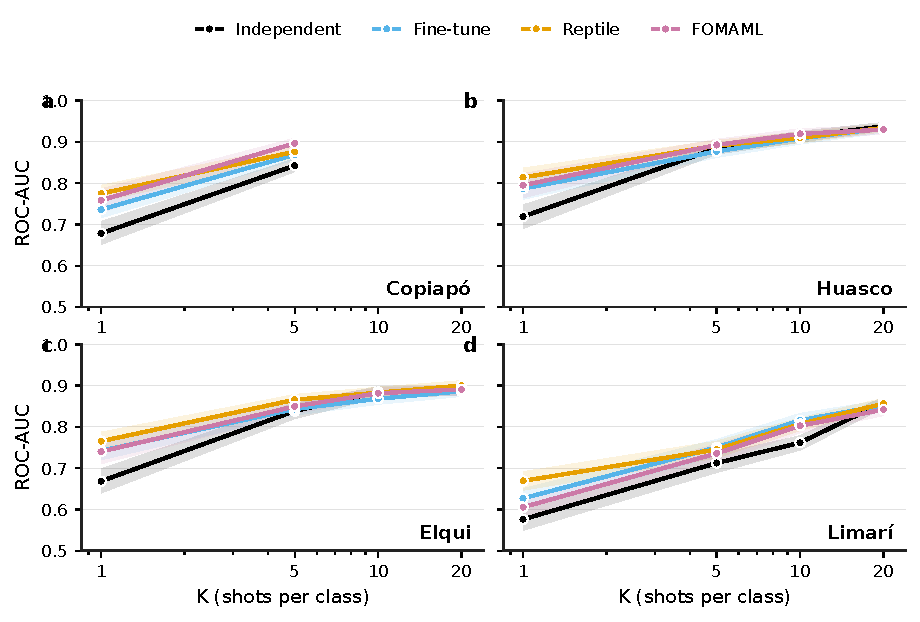
\includegraphics[width=\linewidth]{figS1_auc_vs_k_panel.pdf}
    \caption{ROC-AUC versus $K$ under random cross-validation. Pattern consistent with $F_1$ results in Figure~\ref{fig:f1_random}.}
    \label{fig:auc_random}
\end{figure*}

\begin{figure*}[ht]
    \centering
    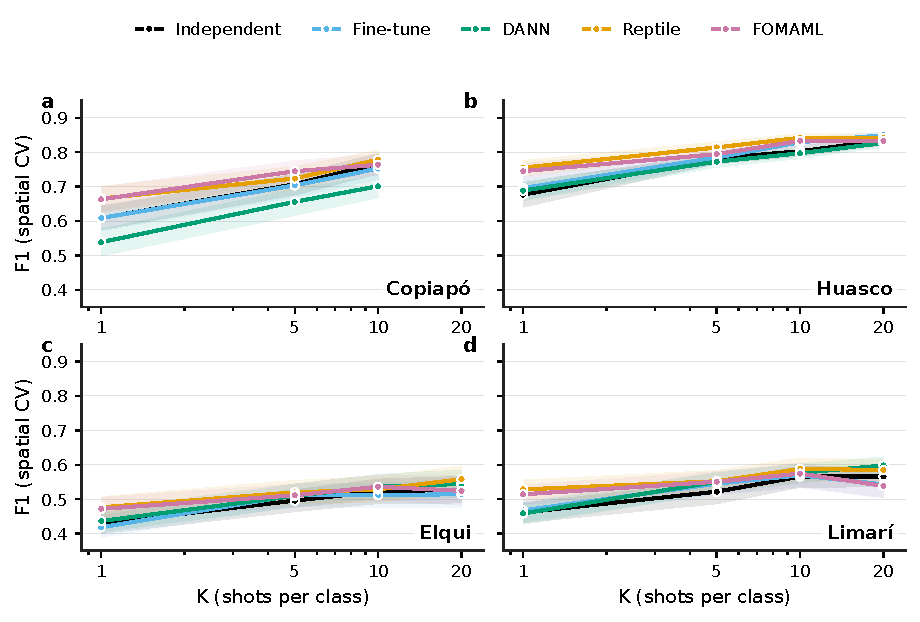
\includegraphics[width=\linewidth]{figS2_spatial_f1_vs_k_panel.pdf}
    \caption{$F_1$ versus $K$ under spatial cross-validation, including DANN. Meta-learning (Reptile or FOMAML) beats Independent at $K=1$ in all four target basins.}
    \label{fig:f1_spatial}
\end{figure*}

\begin{figure*}[ht]
    \centering
    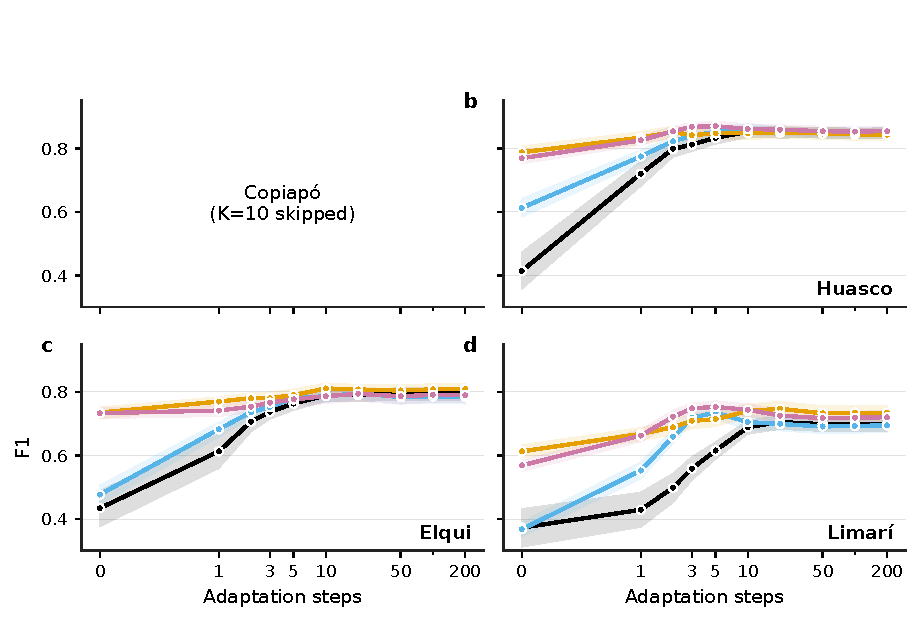
\includegraphics[width=\linewidth]{figS3_adaptation_curves_K10.pdf}
    \caption{Adaptation curves at $K=10$. Same convergence pattern as $K=5$ (Figure~\ref{fig:adaptation}).}
    \label{fig:adapt_k10}
\end{figure*}

\begin{figure*}[ht]
    \centering
    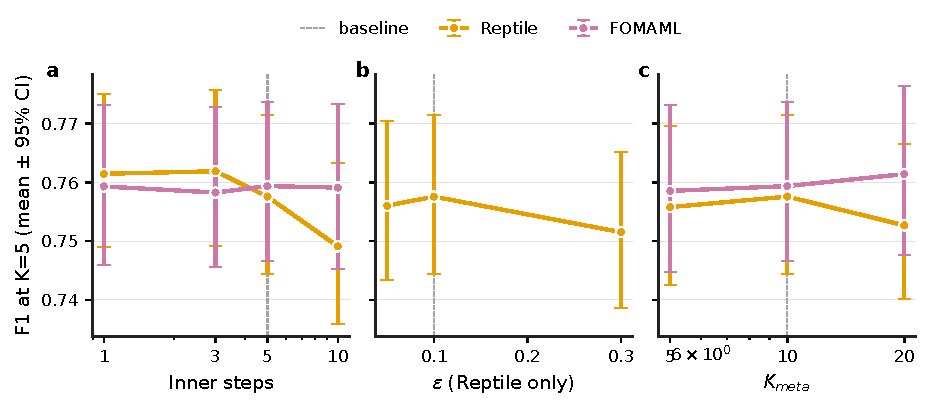
\includegraphics[width=\linewidth]{figS4_ablations.pdf}
    \caption{Hyperparameter sensitivity ablation. (a) Inner gradient steps. (b) Reptile $\epsilon$. (c) Meta-training $K$. Sensitivity is small ($<1$\,pp F1) — baseline configuration is robust.}
    \label{fig:ablations}
\end{figure*}

\begin{figure}[ht]
    \centering
    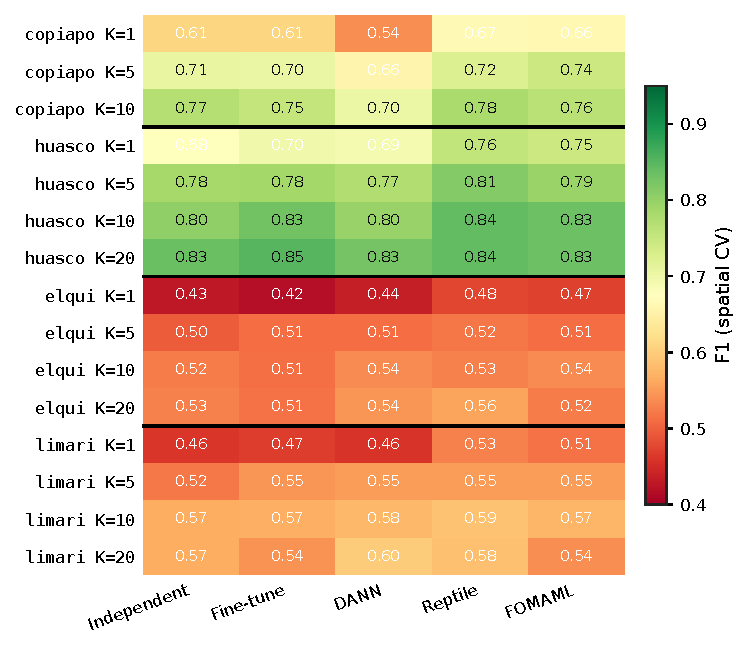
\includegraphics[width=0.6\linewidth]{figS5_summary_heatmap.pdf}
    \caption{$F_1$ (mean) for all (target $\times$ $K$ $\times$ method) combinations under spatial CV.}
    \label{fig:heatmap}
\end{figure}

\begin{figure*}[ht]
    \centering
    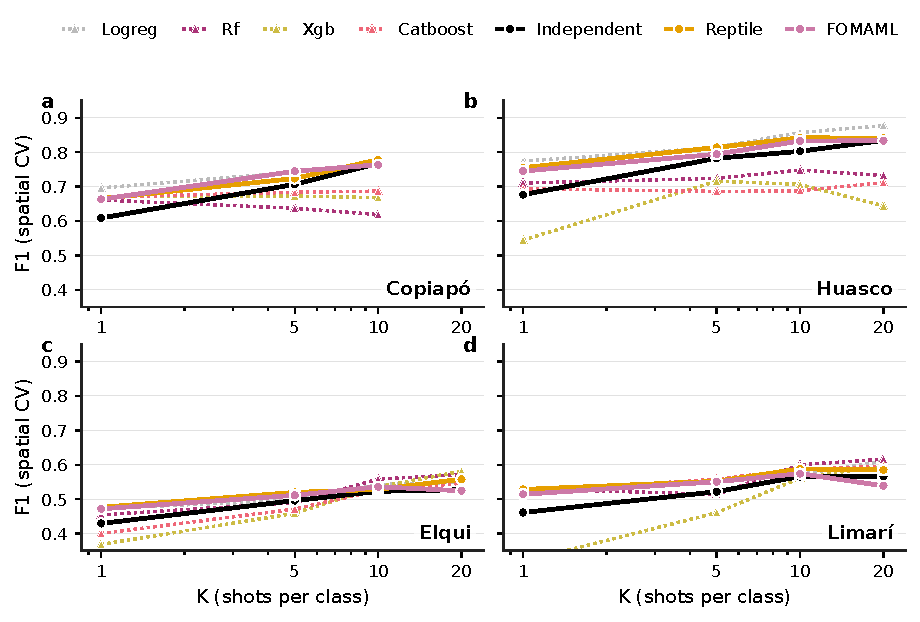
\includegraphics[width=\linewidth]{figS6_classical_vs_meta.pdf}
    \caption{Classical machine learning vs.\ meta-learning under spatial CV. Logistic regression, random forest, XGBoost and CatBoost are competitive with meta-learning in mean $F_1$, but classical models cannot adapt with $K=0$.}
    \label{fig:classical}
\end{figure*}

\begin{figure*}[ht]
    \centering
    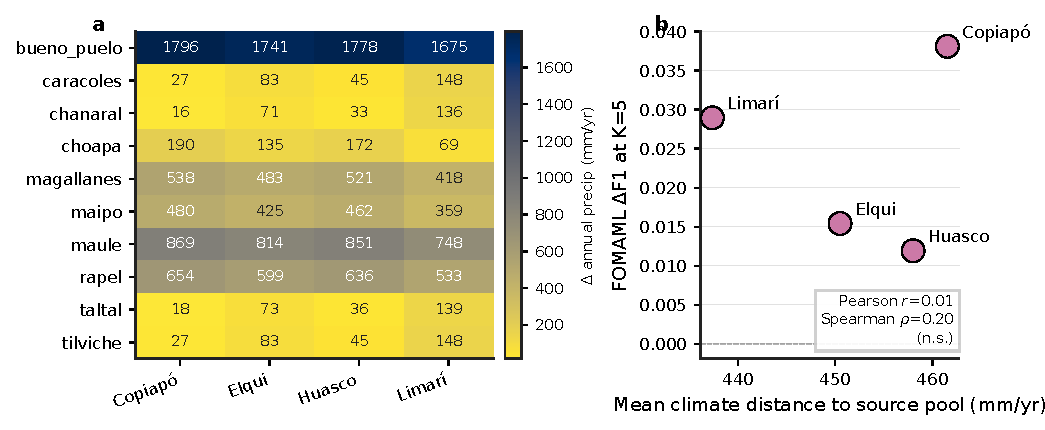
\includegraphics[width=\linewidth]{figS7_climate_distance.pdf}
    \caption{(a) Climate distance matrix between source and target basins (annual precipitation difference). (b) FOMAML transfer advantage at $K=5$ vs.\ mean source-target climate distance; no significant correlation (Pearson $r=0.01$, Spearman $\rho=0.20$).}
    \label{fig:climate}
\end{figure*}

\begin{figure*}[ht]
    \centering
    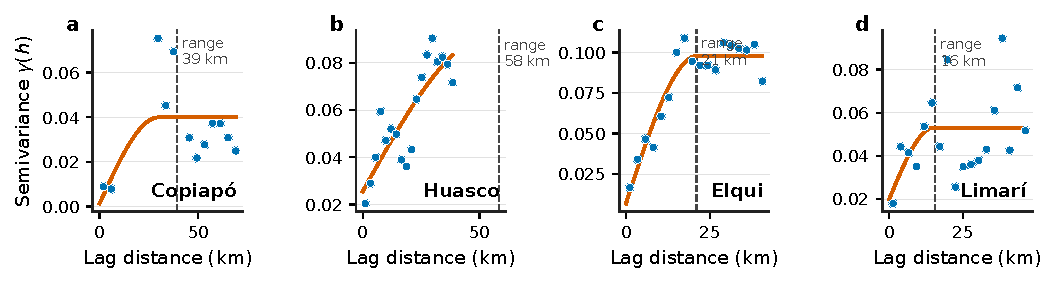
\includegraphics[width=\linewidth]{figS9_variogram.pdf}
    \caption{Empirical variogram of Independent-model residuals for each target basin, with fitted spherical model (red dashed line marks the autocorrelation range). Fitted ranges: 39.3~km (Copiap\'o), 58.5~km (Huasco), 20.9~km (Elqui), 15.6~km (Limar\'i). At $K_{\text{folds}}=5$ the median fold-centroid separation exceeds the range in three of four basins, confirming the spatial folds achieve genuine spatial decorrelation.}
    \label{fig:variogram}
\end{figure*}

\begin{figure*}[ht]
    \centering
    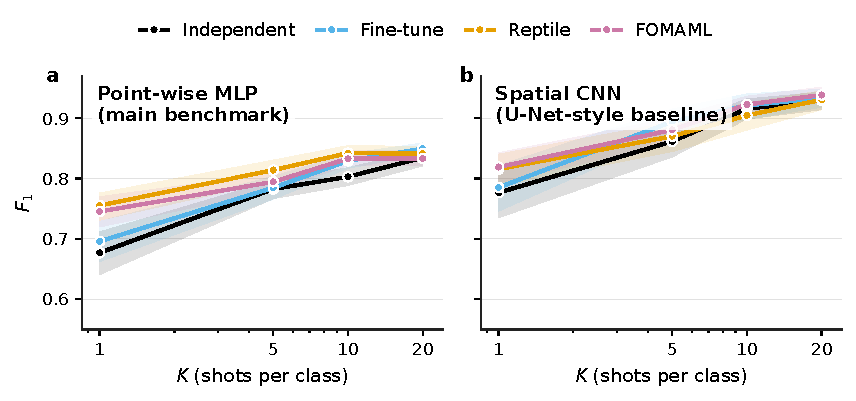
\includegraphics[width=\linewidth]{figS10_unet_vs_mlp.pdf}
    \caption{Spatial CNN (U-Net-style) backbone vs.\ point-wise MLP on Huasco under the same spatial $K$-shot CV protocol with 9 source basins for meta-training. The CNN exceeds the MLP by 6--11~percentage points $F_1$ across all four methods and $K$ values. The meta-learning lift over Independent is smaller in the CNN regime, indicating that spatial context absorbs part of the prediction signal that meta-learning's prior captures in the point-wise setting.}
    \label{fig:cnn}
\end{figure*}

\begin{figure}[ht]
    \centering
    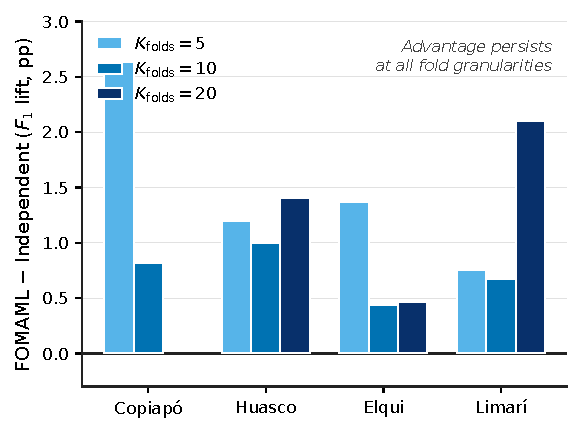
\includegraphics[width=0.7\linewidth]{figS8_kfolds_sensitivity.pdf}
    \caption{FOMAML $-$ Independent mean $F_1$ lift as a function of the number of spatial CV folds $K_{\text{folds}} \in \{5, 10, 20\}$. The meta-learning advantage persists at all fold granularities (lift $+0.4$ to $+2.6$~pp), demonstrating that the reported advantage is not an artifact of the $K_{\text{folds}}=5$ choice.}
    \label{fig:kfolds}
\end{figure}

\end{document}
